\chapter{Problem formulation}
The IPP problem is to plan a path where the agent collects information subject to constraints.
The major difference between this research and conventional IPP is that the agent collects data above a terrain.
The formulation is as follows:
Given the ground set $S$, and $|S| = N$, the goal is to find subgoals that maximize the information subject to the routing constraints.
\begin{equation}
    \max f(X) \\
    s.t. \quad c(X) \le B,
  \label{eq:obj}
\end{equation}
where $X \subseteq S$,  $f$ is informative objective function $f:2^N \rightarrow \mathbb{R}^{+}$, $c$ is the routing cost function $c: 2^N \rightarrow \mathbb{R}^{+},$ and $B$ is the budget. The environment is known, so $f$ and $c$ are oracles that output probability and routing cost values, respectively.

\section{Cost-benefit spanning tree (CBST)}
This problem can be reformulated as a submodular maximization problem.
It can achieve theoretical guarantees via GCB approaches.
If the routing route is tree structure, the theoretical guarantees will be tighter than GCB~\cite{lin2023improvement}.
However, how to find an efficient spanning tree structure is an issue.

No matter how the information-rich vertex is far from the source node or not,
the agent will go to this point using GCB algorithm by traditional shortest path
tree-structured cost function, which is inefficient in search.
If the information-rich vertex is far from the source node,
the agent may not go through this point using GCB algorithm by MST structured cost function.
To solve this issue, the CBST further considers the benefit of $f$.

The cost-benefit spanning tree is similar to Prim-Dijkstra algorithm.
The major difference is that the objective function of CBST is cost-benefit.
The objective function of CBST is
\begin{equation}
\label{equ:cost_benefit_spanning}
  \max(\frac{f(v_j|T)}{\alpha\cdot l_i+d_{ij}}),\quad s.t.\quad v_i \in T, v_j \in V - T,
\end{equation}
where $f$ is accumulated extended probability of detection function, and the other notations are the same with
Eq.~\ref{eq:PD_obj}~\cite{alpert1993direct}.



To illustrate the MST and CBST, an example is shown in Fig.~\ref{fig:ex_epd} and~\ref{fig:GCB_CBST_ex}.
There are $6$ nodes including a source node (index $1$) in the map.
As Fig.~\ref{fig:ex_epd} shows, the black area has less probability than green area after agent went to $v_2$ and scanned the area.
The scanning areas of $v_6$ overlaps that of $v_2$, $v_3$, $v_4$, and $v_5$ since the altitude of $v_6$ is higher than that of $v_2$, $v_3$, $v_4$, and $v_5$.
The probability of each vertex is $p(v_2)=0.25, p(v_3)=0.25, p(v_4)=0.25, p(v_5)=0.25$ and $p(v_6)=1.$
Notice that the total probability is over 1 because there is overlapping.

The tree structure of Fig.~\ref{fig:ex_epd} is shown in Fig.~\ref{fig:GCB_CBST_ex}.
$v_6$ is far from $v_1$ in MST structure (see Fig.~\ref{fig:GCB_CBST_ex}(b)).
On the contrary, $v_6$ is near by $v_1$ in Fig.~\ref{fig:GCB_CBST_ex}(c) in CBST structure.
Under such situations, GCB-CBST performs better than GCB-MST.


On the other hand, the UAV height affects the detection rate.
The glimpse function ($g$) is to describe the relationship between the height and detection rate (see Fig.~\ref{fig:GCB_CBST_ex}(d)).
The $f$ in Eq.~\ref{equ:cost_benefit_spanning} is calculated by $p(v_i)$, path and glimpse function ($g$), where $i \in \{1,...,N\}.$


%In this setting, the MST and CBST algorithms generate Fig.~\ref{fig:GCB_CBST_ex}(b) and Fig.~\ref{fig:GCB_CBST_ex}(c), respectively.
%Assume the budget is $40.$ The agent will go to $v_2,$ and $v_4.$ in GCB-MST, and get accumulated PD: $0.8*0.2+0.8*0.2=0.32$; The agent will go to $v_3$ in GCB-CBST, and get accumulated PD: $0.8*0.6=0.48$.

\begin{figure}[htbp]
 \begin{center}
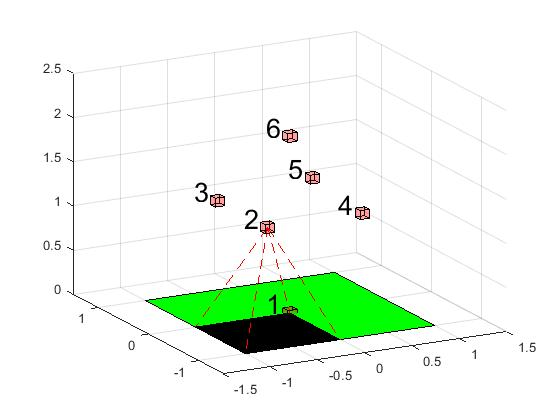
\includegraphics[width=1.0\linewidth]{toy_resol.jpg}
\caption{Illustration of terrain monitoring.
The red cube{\color{olive}s} and decimal numbers represent subgoals and indexes, respectively.
The green and black regions represent lower probability and higher probability, respectively.
}
\label{fig:ex_epd}
 \end{center}
 \end{figure}

\begin{figure}[htbp]
 \begin{center}
\begin{subfigure}{.44\textwidth}
  \centering
  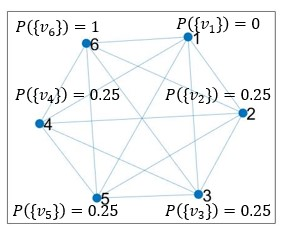
\includegraphics[width=1.0\linewidth]{pt_pd.jpg}
  \caption{Map and subgoals}
\end{subfigure}
\begin{subfigure}{.50\textwidth}
  \centering
  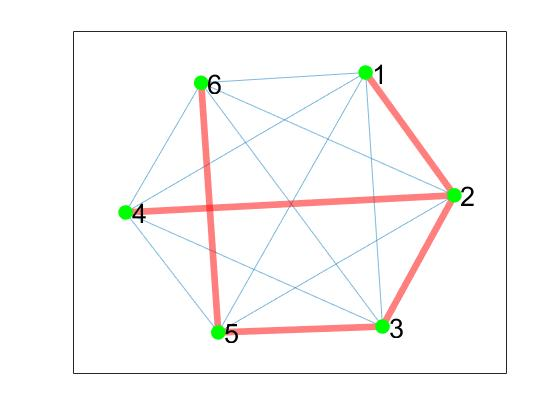
\includegraphics[width=1.0\linewidth]{toy_mst.jpg}
  \caption{Tree structure via MST}
\end{subfigure}
\begin{subfigure}{.50\textwidth}
  \centering
  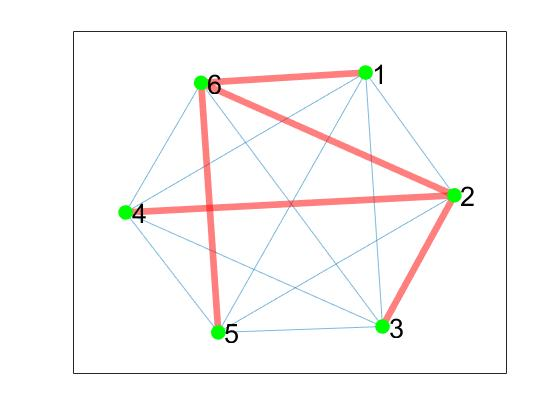
\includegraphics[width=1.0\linewidth]{pt3.jpg}
  \caption{Tree structure via CBST}
\end{subfigure}
\begin{subfigure}{.44\textwidth}
  \centering
  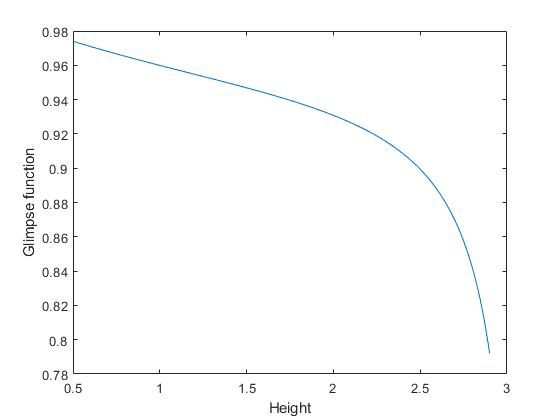
\includegraphics[width=1.0\linewidth]{glimpse.jpg}
  \caption{Glimpse function}
\end{subfigure}
\caption{Example of MST and CBST.
The vertex 1 is the source.
The map is as same as Fig.~\ref{fig:PD_intro} (a).
(a) Map and subgoals.
The blue points, blue edges, function and decimal numbers represent subgoals, paths, probability of each nodes and the index of subgoals, respectively.
(b) Tree structure via MST.
(c) Tree structure via CBST.
(d) Glimpse function ($g$).
%Assume the probability $p_{v_2} = 0.2, p_{v_3} = 0.6, p_{v_4}=0.2,$ and the glimpse function is $0.8.$ The green line is the spanning tree. (a) The graph of all subgoals. (b) Tree structure via MST. (c) Tree structure via CBST.
}
\label{fig:GCB_CBST_ex}
 \end{center}
 \end{figure}



\section{Theoretical bound of CBST}
This section shows the theorems relevant to different kinds of spanning trees.
To introduce the theoretical bound of GCB under tree-structured graphs,
the relationship between the total curvature $\kappa_c$ (see Def.~\ref{def:kappa_f}), the height of tree $H$, and the number of subgoals are as follows:
%the total curvature, and largest size of feasible solution are defined as follows:

%\begin{definition}[Submodularity ratio~\cite{zhang2016submodular}]
%Given a non-negative set function $f$, the submodularity ratio of $f$ is defined as
%
%\begin{equation}
%\alpha_f=\min_{S_A\subseteq S_B, s\notin S_B} \frac{f(S_A \cup s) - f(S_A)}{f(S_B \cup s) - f(S_B)}.
%\end{equation}
%
%The two properties of $\alpha_f$ holds: \\
%1. $0 \le \alpha_f \le 1.$ \\
%2. $f$ is submodular if and only if $\alpha_f = 1.$ \\
%
%\label{def:sub_ratio}
%\end{definition}

According to Thm.~\ref{thm:GCB_lin}, the tighter theoretical bound is relevant to ($\kappa_c$).
The $\kappa_c$ of SPT and MST under constraints are proved as follows:

\begin{theorem} [$\kappa_c$ in tree structure~\cite{SHIEH2023}]
{Given the tree structure of the cost function $c$, then $\kappa_c$ either equal to $0$ or $1$.
}
\label{thm:kappa}
\end{theorem}

%\begin{proof}
%{\color{olive}
%  Skip. \\
%  The proof refers to Rex-Shieh's thesis.
%  }
%\end{proof}


%\begin{definition}[{\color{olive}The height of the tree and the depth of a node}]
%{\color{olive}The height of the tree is the length of the longest downward path to a leaf from root.
%The depth of a node is the length of the path to its root.}
%\label{def:height_tree}
%\end{definition}
%
%{\color{olive}
%For example, the height of tree in Fig.~\ref{fig:GCB_CBST_ex} (b) is 4 (($v_1\rightarrow v_2\rightarrow v_3\rightarrow v_5\rightarrow v_6$) four edges) and the depth of $v_5$ in Fig.~\ref{fig:GCB_CBST_ex} (b) is 3 (($v_1\rightarrow v_2\rightarrow v_3\rightarrow v_5$) three edges).}

Since the $\kappa_c$ in tree structure is equal to $1$ or $0$,
the subsequent theorems focus on on exploring the relationship between $\kappa_c$ and the height of the tree $(H)$.

\begin{theorem}[The relationship between $\kappa_c$ and the height of trees]
Given the tree structure of the cost function and the height of the tree ($H$), \\
if $H=1$, $\kappa_c = 0$;\\
if $H>1$, $\kappa_c = 1$.
%Given the tree structure of the cost function $c$, and the height of tree is equal to $1$, then $\kappa_c = 0.$
%}
\label{thm:kappac}
\end{theorem}

\begin{proof}

W.L.O.G., we assume $v_1$ is the source node.\\
\\
Case $1$: ($H=1$)\\
$\because$ $H=1$. \\
$\therefore\forall v_i$ are only connecting $v_1$, where $i\in\{2,...,n\}$, $n$ is the amount of nodes.\\
$\Rightarrow c(v_i) = ||v_i-v_1||, i \in \{2,...,n\}$ \\
$\Rightarrow \kappa_c = 0$ ( Eq.~\ref{eq:kappa} )\\
\\
Case $2$: ($H> 1$)\\
%$\because$ the tree height $> 1$ \\
$\therefore \exists$ the height is equal to 2 or greater than 2. \\
Since the case of $H>2$ includes the case of $H=2$,
only the case that the height is 2 will be proved.\\
W.L.O.G., assume $v_2$ is the node of depth $= 1$, $v_3$ is the node of depth $= 2,$ and the node between $v_1$ and $v_3$ is $v_2$. \\
Let $S=\{v_1, v_2, v_3\}$, and $s = \{v_2 \}$ \\
$\because c(S) = 2*(||v_1-v_2||+||v_3-v_2||)$ and \\
$\begin{aligned}[t]
    c(S\setminus\{s\}) &= 2*||v_1-v_3|| \\
      &= 2*(||v_1-v_2||+||v_3-v_2||) \\
\end{aligned}$
\\
The first equation is by definition, and the second one is by the tree structure. \\ There is only one path between $v_1$ and $v_3.$\\
$\therefore c(S\setminus\{s\}) = c(S)$ \\
By definition of $\kappa_c$ (Eq.~\ref{eq:kappa}), \\
$\min_{s\in S:f(\{ s \}) > 0}\frac{f(S)-f(S\setminus\{ s\})}{f(\{s\})} = 0$\\
$\therefore \kappa_c = 1$ \\


\end{proof}

\begin{theorem} [$\kappa_c$ in SPT]
Given an empty map and the shortest path tree structure of the cost function $c$, then $\kappa_c = 0$.
\label{thm:spt}
\end{theorem}


\begin{proof}
Given a complete graph $G=(V, E), V=\{ v_1,...,v_n \}$ \\
$\because\forall i \ne j \ne k\in\{1,...,n\}, ||v_k-v_i||+||v_i-v_j||\ge||v_k-v_j||$ \\
the equality only holds in the $v_i,v_j,$ and $v_k$ in a straight line. \\
$\therefore$The height of shortest spanning tree is $1$, i.e. the number of maximal edge between the source node and the others is $1$.\\
$\because$ the height of shortest spanning tree is $1$.\\
%$\therefore f(S\setminus\{s\}) = f(S)-f(\{s\}) $, where $s \in S.$\\
$\therefore$ by Thm.~\ref{thm:kappac}, $\kappa_c  = 0$ \\
%According to the definition of $\kappa_f$ in Eq.~\ref{def:K_c}, $\kappa_c = 0.$

\end{proof}

As~Fig.~\ref{fig:spt_thm} shows, the vertex $1$ is the source node, and the others will be in level $2$ due to triangle inequality.

\begin{figure}[htbp]
  \centering
  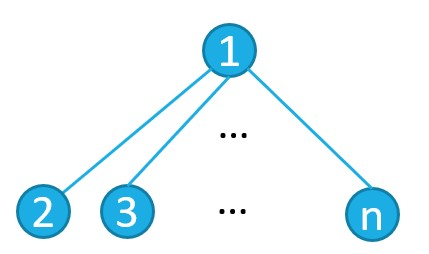
\includegraphics[width=0.6\linewidth]{spt_.jpg}
  \caption{Illustration of tree height of Thm.~\ref{thm:spt}}
  \label{fig:spt_thm}
\end{figure}

\begin{figure}[htbp]
 \begin{center}
\begin{subfigure}{.33\textwidth}
  \centering
  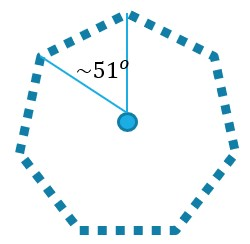
\includegraphics[width=1.0\linewidth]{51.jpg}
  \caption{Regular heptagon}
\end{subfigure}
\begin{subfigure}{.36\textwidth}
  \centering
  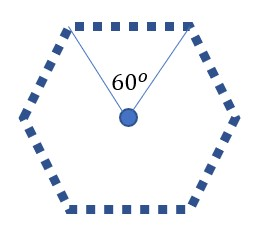
\includegraphics[width=1.0\linewidth]{60.jpg}
  \caption{Hexagon}
\end{subfigure}
\caption{Illustration of minimum numbers of Thm.~\ref{thm:mst}
}
\label{fig:mst_thm}
 \end{center}
 \end{figure}

%\begin{lemma}[{\color{olive} Maximum number of vertices in 2D}]
%If the number of vertices is greater than $7$, $\exists j,k \in \{1,...,n\}, ||v_1-v_j||>||v_j-v_k||$:
%{\color{red} (use a lemma or corollary and give a number for refer...)}
%\label{lem:vertices7}
%\end{lemma}
%
%\begin{proof}
%W.L.O.G., we assume $v_1$ is the source node.\\
%We use proof by contradiction. \\
%$\forall j,k \in \{1,...,n\}, ||v_1-v_j||\le||v_j-v_k||,$ then the number of vertices is less than $8$. \\
%It represents $\angle v_j v_1 v_k\ge 60^{\circ}$, $\forall j \ne k \in\{1,...,n\}$  \\
%It's obviously in Fig.~\ref{fig:mst_thm}(b).\\
%$\therefore$ If the number of vertices is greater than $7$, $\exists j,k \in \{1,...,n\}, ||v_1-v_j||>||v_j-v_k||.$
%
%
%\end{proof}

%\begin{lemma}[{\color{olive} The relation between $\kappa_c$ and the height of tree = 1}]
%Given the tree structure of the cost function $c$, and the height of tree is greater than $1$, then $\kappa_c = 1.$
%\label{lem:kappac1}
%\end{lemma}

To investigate the relationship between $\kappa_c$ and the number of subgoals,
the kissing number problem is introduced for the proof.
The kissing number problem investigates the maximum number of non-overlapping spheres that can touch a central sphere in a given space.
It aims to determine the highest possible number of points on the surface of a sphere that can be equidistant from a fixed central point.


%{\color{red} (Could you write "the height of tree" to $\kappa_c = 0$ and $\kappa_c = 1$ in a theorem and prove it.)}

%\begin{proof}
%{\color{olive}$\because$ the tree height $> 1$ \\
%$\therefore \exists$ the height is equal to 2 or greater than 2. \\
%We will prove the height is 2, because the height is greater than 2 is similar.\\
%W.L.O.G., assume $v_1$ is source node, $v_2$ is the node of height $= 1$, $v_3$ is the node of height $= 2,$ and the node between $v_1$ and $v_3$ is $v_2$. \\
%We take $S=\{v_1, v_2, v_3\}$, and $s = \{v_2 \}$ \\
%$\because c(S) = 2*(||v_1-v_2||+||v_3-v_2||)$ and \\
%$\begin{aligned}[t]
%    c(S\setminus\{s\}) &= 2*||v_1-v_3|| \\
%      &= 2*(||v_1-v_2||+||v_3-v_2||) \\
%\end{aligned}$
%\\
%The first equation is by definition, and the second one is by tree structure. There is only one path between $v_1$ and $v_3.$\\
%$\therefore c(S\setminus\{s\}) = c(S)$ \\
%By definition of $\kappa_c$ (Eq.~\ref{eq:kappa}), \\
%$\min_{s\in S:f(\{ s \}) > 0}\frac{f(S)-f(S\setminus\{ s\})}{f(\{s\})} = 0$\\
%$\therefore \kappa_c = 1$
%}
%
%
%\end{proof}

\begin{theorem} [$\kappa_c$ in MST]
Given an empty map and the minimum spanning tree structure (MST) of the cost function $c$, the $\kappa_c = 1$ when\\
\begin{equation}
(i) |S| > 7\; in\; 2D\; environments; \\
\label{eq:2D}
\end{equation}
\begin{equation}
(ii) |S| > 10\; in\; 3D\; environments.
\label{eq:3D}
\end{equation}
\label{thm:mst}
\end{theorem}

\begin{proof}
Given complete graph $G=(V, E), V=\{ v_1,...,v_n \}$ \\
W.L.O.G., we assume $v_1$ is the source node.\\
\\
Case (i): 2D environments\\
Proof by contradiction is as follows. \\
$|S| \le 7$ in 2D environment. \\
The subgoals are arranged in the pattern of vertices of a hexagon, and the source node is in the center of a hexagon. \\
\begin{equation}\label{eq:mst}
  \therefore\forall j,k \in \{1,...,n\}, ||v_1-v_j||\le||v_j-v_k||.
\end{equation}
%$\forall j,k \in \{1,...,n\}, ||v_1-v_j||\le||v_j-v_k||.$ \\
By Eq.~\ref{eq:mst} and the property of MST, the height of MST is equal to 1. \\
$\Rightarrow \kappa_c = 0.$ (by Thm.~\ref{thm:kappac})\\
%$\rightarrow\leftarrow$ \\
Hence, $|S| > 7.$\\
%$\forall j,k \in \{1,...,n\}, ||v_1-v_j||\le||v_j-v_k||,$ then the number of vertices is less than $8$. \\
%It represents $\angle v_j v_1 v_k\ge 60^{\circ}$, $\forall j \ne k \in\{1,...,n\}$  \\
%It's obviously in Fig.~\ref{fig:mst_thm}(b).\\
%$\therefore$ If the number of vertices is greater than $7$, $\exists j,k \in \{1,...,n\}, ||v_1-v_j||>||v_j-v_k||.$
%
%
%By Lemma.~\ref{lem:vertices7} and the property of MST, if the number of subgoals greater than $7,$ the height of MST is greater than $1$.\\
Case (ii): 3D environments\\
This problem can be seen as  \\
%finding the maximum number of points, where the distances between these points are greater than the distances between these points and root.}
$\max (N)$ s.t. $ ||v_1-v_j||\ge||v_j-v_k||, j,k\in\{ 1,...,N \} $.
When $n > N$, it represents $H > 1$ $\Rightarrow \kappa_c = 1$
%{\color{red}???? Define the notations and denote them in the figure (e.g., distances between these points , the distances between these points and root).}


It is similar to the kissing number problem.
$k(d)$ denotes the highest number of non-overlapping spheres in $\mathbb{R}^d$ that can touch another sphere of the same size. $k(3)=12$ has been proved~\cite{schutte1952problem}.
The relationship between the kissing balls and the tree is as follows:
As shown in Fig.~\ref{fig:mst_thm_overlapping} and~\ref{fig:mst_thm_3D},
the central sphere ($r_1$) represents the root of the tree.
The highest possible number of points on the surface of a sphere ($r_1,...,r_N$) corresponds to the number of points ($N$) (see Fig.~\ref{fig:mst_thm_overlapping}(a)).
The overlapping spheres correspond to the distances between these points (green lines) are smaller than the distances between these points and root (blue lines) (see Fig.~\ref{fig:mst_thm_overlapping}(b)).
%{\color{red} (How about plotting a figure to illustrate it.)}


The source node is placed on the surface ($x=y=z=0$), and the other nodes are placed above the surface ($x \in \mathbb{R}, y\in \mathbb{R}$ and $z \ge 0$).
%$\therefore$ The kissing problem is considered in $\mathbb{R}^{2.5}$.\\
%In other words, the subgoals are above xy plane.\\
First, there are at most six points in xy plane (see Fig.~\ref{fig:mst_thm_3D}(a)).
Second, since $k(3)=12$, the kissing number in the upper xy plane and in lower xy plane are $3$ and $3$, respectively (see Fig.~\ref{fig:mst_thm_3D}(b)). It represents $v_2,...,v_7$ are points in xy plane, and $v_8, v_9, v_{10}$ are upper xy plane. $\because$ There are no overlapping spheres. \\
$\Rightarrow ||v_1-v_j||\le||v_j-v_k||, \forall j \ne k \in\{2,...,10\}$ \\
Finally, there are six balls in xy plane and three balls above xy plane.\\
$\Rightarrow$ there are $9$ balls satisfying conditions. \\
%If there are $10$ balls, the balls are overlapping.
%It means the distance of the centers of two overlapping balls is smaller than the distance of the centers of the other non-overlapping balls. \\
$\Rightarrow$ the height of MST is greater than $1$ if the number of subgoals greater than $10$ (including root) in a three-dimension environment. \\
$\Rightarrow$ $\kappa_c = 1.$


%An empty map represents the graph of cost function as a complete graph. The minimum spanning tree is to find the minimum weighting in the spanning tree. The weighting is the distance between two subgoals. If the weighting between the source and another node is smaller than the distance between another node and the other nodes, the height of MST is $2$ possibly. If the number of subgoals is greater than $6$, the weighting of the existing two subgoals is less than the weighting of the source and one of them. The height of MST is more than $1$, so the $\kappa_c = 1$.



\end{proof}

\begin{figure}[htbp]
  \centering
  \begin{subfigure}{.4\textwidth}
  \centering
  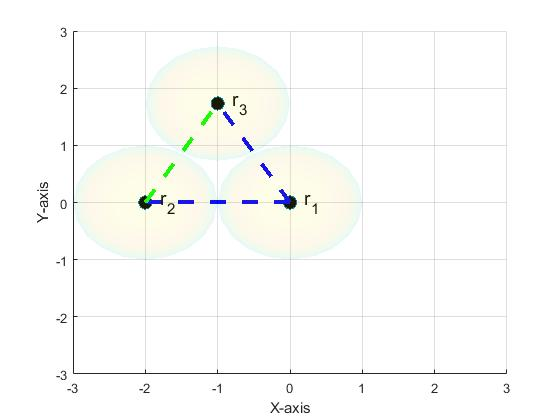
\includegraphics[width=1.0\linewidth]{thm5_1.jpg}
  \caption{Non-overlapping}
\end{subfigure}
\begin{subfigure}{.4\textwidth}
  \centering
  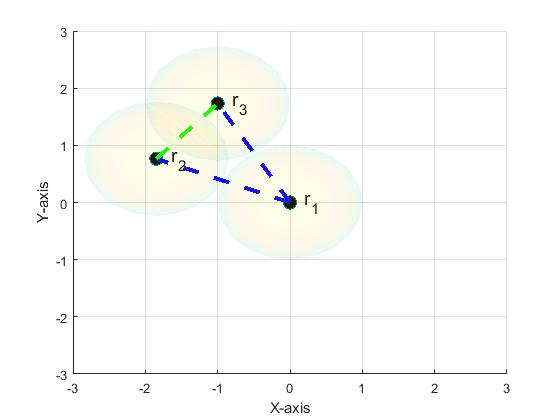
\includegraphics[width=1.0\linewidth]{thm5_2.jpg}
  \caption{Overlapping}
\end{subfigure}
  \caption{Illustration of overlapping balls in Thm.~\ref{thm:mst}.
  The black points, the decimal numbers, the blue lines, and the green line(s) represent the subgoals, the indexes of subgoals, the distance between source node ($r_1$) and the other nodes ($r_2, r_3$), and the distance between the other nodes ($r_2$ and $r_3$), respectively.
  (a) The non-overlapping case.
  (b) The overlapping case.
  }
  \label{fig:mst_thm_overlapping}
\end{figure}

\begin{figure}[htbp]
  \centering
  \begin{subfigure}{.4\textwidth}
  \centering
  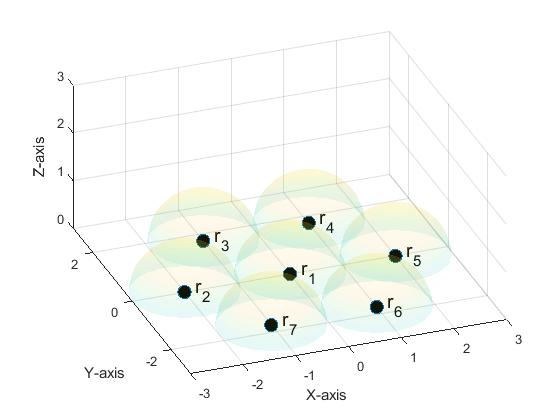
\includegraphics[width=1.0\linewidth]{3D.jpg}
  \caption{The center of balls in $z=0$}
\end{subfigure}
\begin{subfigure}{.4\textwidth}
  \centering
  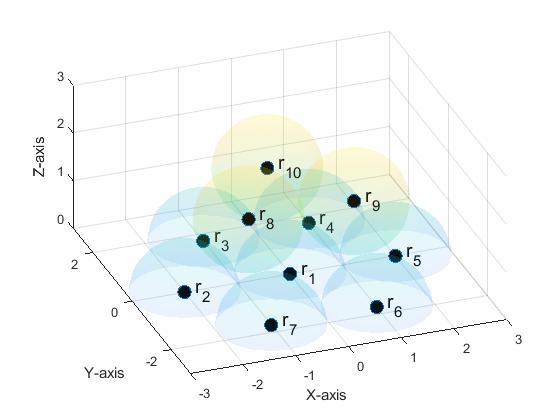
\includegraphics[width=1.0\linewidth]{3D_plus.jpg}
  \caption{The center of balls in $z\ge 0$}
\end{subfigure}
  \caption{Illustration of kissing balls of Thm.~\ref{thm:mst}}
  \label{fig:mst_thm_3D}
\end{figure}

To give examples of the proofs, 2D and 3D cases are as follows:
As Fig.~\ref{fig:mst_thm}(a) shown, the source node is at the intersection point between two solid lines.
If the edges of graph are $7$ and the subgoals are the vertices of regular heptagon, the solid blue line is greater than the dashed line.
It implies that if $|S| > 7$, $H>1$ for MST;
If the number of graph edges is $6$ and the subgoals are in the vertices of hexagon,
the solid blue line is less than or equal to the dashed line in Fig.~\ref{fig:mst_thm}(b).
It implies that if $|S| = 7$, $H=1$ for MST.

Note that if $|S|\le 10$ in 3D environment, either $\kappa_c = 0$ or $\kappa_c = 1$ is possible.
As Fig.~\ref{fig:GCB_CBST_ex} shows, there are $6$ nodes in graph.
The height of MST in Fig.~\ref{fig:GCB_CBST_ex} is $4$, i.e., $\kappa_c = 1$.

As Fig.~\ref{fig:mst_thm_3D}(a) shows, there are at most six non-overlapping balls in xy plane.
By $k(3) = 12$~\cite{schutte1952problem}, there are three centers upper xy-plane (see Fig.~\ref{fig:mst_thm_3D}(b)).
There are at most $10$ points (including central point) satisfying $||v_1-v_j||\le||v_j-v_k||, \forall j \ne k \in\{2,...,10\}$.

%{\color{red}To be done after completing Thm.~\ref{thm:mst} (ii).}


%{\color{red} (Write a theorem including MST and SPT bound to save space since they are similar.
%Notice their assumptions!)}

\begin{theorem} [The theoretical guarantees of GCB-SPT and GCB-MST]
By Thm.~\ref{thm:spt} and Thm.~\ref{thm:mst}, given a submodular monotone set function $f,$
a minimum spanning tree cost function $c_{MST}$ with the condition of subgoals,
and a shortest path tree cost function $c_{SPT}$,
the GCB approach is to maximize f subject to the budget $B$.
The performance of a set $X$ with $c_{MST}$ and of a set $X$ with $c_{SPT}$ achieve
\begin{equation}
  f(X)\ge\frac{1}{2}(1-\frac{1}{e})f(X_{MST}),
\end{equation}
and
\begin{equation}
  f(X)\ge\frac{1}{2}(1-\frac{1}{e})f(X_{SPT}),
\end{equation}
where
\begin{equation}
 X_{MST} = arg\max _X\{
f(X) | c_{MST}(X)\le B (\frac{1}{K_{c_{MST}}})
\},
\label{eq:SPT_k}
\end{equation}
and
\begin{equation}
 X_{SPT} = arg\max _X\{
f(X) | c_{SPT}(X)\le B
\},
\label{eq:MST_k}
\end{equation}
respectively.

\begin{proof}
Case1: The theoretical guarantees of GCB-MST is as follows:\\
By Thm.~\ref{thm:mst}, if the subgoal condition is satisfied, $\kappa_{c}=1$.
Substituting  $\kappa_{c}=1$ into Eq.~\ref{eq:OPT_lin}, the budget constraint is $c(X)\le B(\frac{1}{K_{c_{MST}}})$\\
$\therefore X_{MST} = arg\max _X\{
f(X) | c_{MST}(X)\le B (\frac{1}{K_{c_{MST}}})
\}$\\
Case2: The theoretical guarantees of GCB-SPT is as follows:\\
By Thm.~\ref{thm:spt}, the $\kappa_{c}$ of SPT is 0.\\
Substituting  $\kappa_{c}=0$ into Eq.~\ref{eq:OPT_lin}, the budget constraint is $c(X)\le B)$\\
$\therefore X_{SPT} = arg\max _X\{
f(X) | c_{SPT}(X)\le B
\}$


\end{proof}
%{\color{red} (Check the notation of c, c hat. Make it coherent!)}
%{\color{olive}Note that taking $\kappa_c = 0$ or $1$ to Eq.~\ref{eq:OPT_lin} can get the Eq.~\ref{eq:SPT_k} and Eq.~\ref{eq:MST_k}.}

%{\color{red} (Write a short proof via EQ5 in the case of $\kappa_c =0 or 1$.)}

\label{thm:sptmstGCB}
\end{theorem}

%\begin{theorem}
%By Thm.~\ref{thm:mst}, given a submodular monotone set function $f$ and a minimum spanning tree cost function $c$,
%the GCB approach is to maximize f subject to the budget $B$.
%The performance of a set X achieves
%\begin{equation}
%  f(X)\ge\frac{1}{2}(1-\frac{1}{e})f(\overline{X}),
%\end{equation}
%where
%\begin{equation}
% \overline{X} = arg\max _X\{
%f(X) | c(X)\le B (\frac{1}{K_c})
%\}.
%\label{eq:OPT_MST}
%\end{equation}
%\label{thm:mstGCB}
%\end{theorem}


\begin{corollary} [The theoretical guarantees of GCB-CBST]
Given a submodular monotone set function $f$, a CBST cost function $\overline{c}$ with $\alpha = 0$ and Eq.~\ref{eq:2D}, Eq.~\ref{eq:3D}, and a CBST cost function $\breve{c}$ with $\alpha = 1,$
the GCB approach is to maximize f subject to the budget $B$ in the case of IPP on the terrain.
The performances of a set X achieve
\begin{equation}
  f(X)\ge\frac{1}{2}(1-\frac{1}{e})f(\overline{X}),
\end{equation}
and
\begin{equation}
  f(X)\ge\frac{1}{2}(1-\frac{1}{e})f(\breve{X}),
\end{equation}
where
\begin{equation}
 \overline{X} = arg\max _X\{
f(X) | \overline{c}(X)\le B (\frac{1}{K_{\overline{c}}})
\}.
\label{eq:OPT_CBST_alpha0}
\end{equation}
and
\begin{equation}
 \breve{X} = arg\max _X\{
f(X) | \breve{c}(X)\le B
\}.
\label{eq:OPT_CBST_alpha1}
\end{equation}
, respectively.
\label{thm:CBSTGCB}
\end{corollary}


\begin{proof}
The numerator of the CBST objective function is fixed (see Eq.~\ref{equ:cost_benefit_spanning}).
When $\alpha=0$, denominator of the CBST objective function is the same as that of the MST;
when $\alpha=1$, denominator of the CBST objective function is the same as that of the SPT.
Hence, the theoretical guarantee is the same as Eq.~\ref{eq:SPT_k} and Eq.~\ref{eq:MST_k}.\\
  
\end{proof}
%{\color{red} (If it is the same with Theorem, Don't repeat it again. Only describe it.)}

Although the theoretical guarantees of CBST is the same as MST, the performance of CBST is different from that of MST due to objective function of the tree spanning.
The problem is with budget constraints.
The CBST spans the tree adopts cost-benefit objective, so the agent will go through the subgoal with more cost-benefit ratio than that of MST.
For example, the budget is $3$ and the budget constraint is routing in Fig.~\ref{fig:method_intro}(a)
, the path in GCB-MST is $\{1, 2, 3 \}$ and the path in GCB-CBST is $\{1,6,5 \}$ in Fig.~\ref{fig:toy_mst_cbst}(a)(b).
The accumulated EPD in GCB-MST is $0.48$ and that in GCB-CBST is $0.95.$

%{\color{red} (You should have more description about this theorem. The bound is the same.
%You should explain or prove why it is better (e.g., routing cost))}






\begin{figure}[htbp]
 \begin{center}
\begin{subfigure}{.44\textwidth}
  \centering
  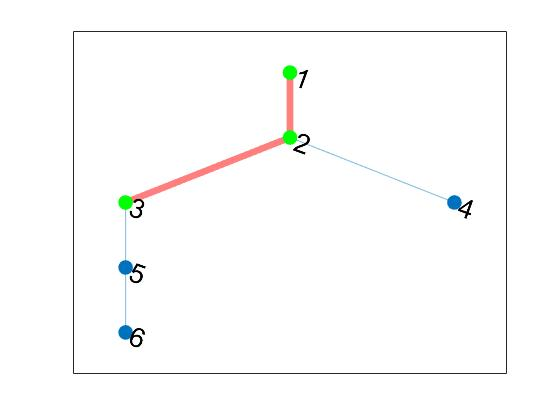
\includegraphics[width=1.0\linewidth]{toy_mst_path.jpg}
  \caption{Path in GCB-MST}
\end{subfigure}
\begin{subfigure}{.44\textwidth}
  \centering
  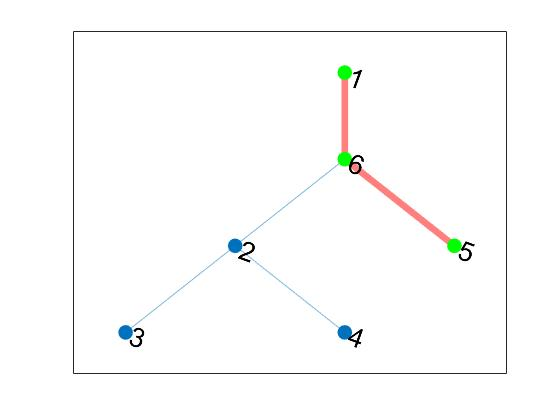
\includegraphics[width=1.0\linewidth]{toy_cbst_path.jpg}
  \caption{Path in GCB-CBST}
\end{subfigure}
\caption{Example of difference between GCB-MST and GCB-CBST}
\label{fig:toy_mst_cbst}
 \end{center}
 \end{figure} 